\documentclass[a4paper,10pt,twocolumn]{ltjsarticle}
\usepackage[haranoaji]{luatexja-preset}
\usepackage[top=18mm,bottom=20mm,left=17mm,right=17mm,columnsep=8mm]{geometry}
\usepackage{graphicx,booktabs,array,caption,enumitem,xcolor,tikz}
\usetikzlibrary{shapes.geometric}
\setlength{\parindent}{1\zw}
\renewcommand{\baselinestretch}{1.0}
\setlength{\parskip}{0pt}
\renewcommand{\thesection}{\arabic{section}.}
\renewcommand{\thesubsection}{\arabic{section}.\arabic{subsection}.}
\makeatletter
\renewcommand{\section}{\@startsection{section}{1}{\z@}{1.1\Cvs \@plus.4\Cdp \@minus.2\Cdp}{.5\Cvs \@plus.2\Cdp}{\normalfont\gtfamily\bfseries\large}}
\renewcommand{\subsection}{\@startsection{subsection}{2}{\z@}{.8\Cvs \@plus.3\Cdp \@minus.2\Cdp}{.3\Cvs \@plus.1\Cdp}{\normalfont\gtfamily\bfseries\normalsize}}
\makeatother
\captionsetup{font={small,sf},labelsep=space,justification=raggedright,singlelinecheck=false,skip=3pt}
\captionsetup[table]{position=top}
\setlist[itemize]{leftmargin=1.2\zw,itemsep=0pt,topsep=2pt,parsep=0pt}
\setlength{\textfloatsep}{8pt plus 2pt minus 2pt}
\setlength{\floatsep}{8pt plus 2pt minus 2pt}
\setlength{\intextsep}{8pt plus 2pt minus 2pt}
\pagestyle{plain}
\raggedbottom
\begin{document}
\twocolumn[{
\noindent\fbox{\gtfamily\small\ 生成AI論文\ }\par\medskip
\begin{center}
{\gtfamily\bfseries\LARGE ICTスキルの男女差は，国によってどれだけ違うのか：表計算とプレゼン資料作成を，日本と他の国・地域で比べる$^{\dagger}$}\par\medskip
{\gtfamily\bfseries\large 表計算とプレゼン資料作成における男女差（男性−女性）の国際比較と日本の位置}\par\medskip
{\normalsize EduData調査研究グループ$^{*1}$・教育データサイエンス解析班$^{*2}$}\par
{\small オープン教育統計推進プロジェクト$^{*1}$・初等中等STEM教育データ基盤ユニット$^{*2}$}
\end{center}\smallskip
\noindent\begin{minipage}{\textwidth}\small UNESCO統計研究所（UIS）の2021年の公表値を用い，表計算ソフトでの算術式の使用とプレゼン資料の作成について，男女差（男性−女性，\%ポイント）を国・地域間で比べ，日本の位置を調べた．男女差を求められた38の国・地域で，表計算の男女差は-4.1から18.8，プレゼン資料作成の男女差は-14.9から17.4に分布し，日本は表計算で16.3（大きい側から3番目），プレゼン資料作成で15.0（同2番目）であった．2つの男女差は，両方が求められた36の国・地域で正の関連を示し（\textit{r}=.75，95\%CI [0.57, 0.87]，\textit{BF}\textsubscript{10}>1000），日本とマレーシアを除いても残った（\textit{r}=.63）．結果は国・地域の集計値の記述であり，個人の因果や理由は示さない．\par\smallskip
\noindent{\gtfamily キーワード：}UNESCO，ICTスキル，男女差，国際比較\end{minipage}\medskip
}]
\let\thefootnote\relax
\footnotetext{\footnotesize 2026年10月執筆\\ $^{\dagger}$How Do Gender Gaps in ICT Skills Differ by Country? Comparing Spreadsheet and Presentation Skills in Japan and Other Countries†\\ $^{*1}$ Open Education Data Project, Tokyo, Japan\quad $^{*2}$ Educational Data Science Unit, Tokyo, Japan}
\section{はじめに}
\subsection{研究の背景}
ICTスキルをもつ若者・成人の割合は，SDG 4.4.1の指標として国際的に集計されている．元の統計はITU (2023)が各国の世帯調査などから集めたものである．UNESCO (2023)は教育での技術の利用を「誰の条件で」用いるのかという観点から検討しており，デジタルな資源や技能の差を論じる枠組みとして，Ragnedda (2018)のデジタル資本やvan Dijk (2020)のデジタルデバイドがある．こうした議論を背景にすると，技能の男女差が国・地域によってどの程度違うかは，まず記述として確かめておく価値がある．

表計算ソフトでの算術式の使用とプレゼン資料の作成は，学校でも職場でも使われる基本的な操作である．Wing (2006)は計算的思考を論じたが，本研究の指標は個別の操作の経験であり，計算的思考そのものを測るものではない．Hubwieser et al. (2015)は初等中等教育での情報科学教育の国際的な現状を整理した．国によって情報教育の位置づけが異なることが男女差の違いと関わるかは，教育課程のデータをもたない本研究では確かめられない．

本研究は，UISが公表する2021年の値を用い，国・地域間の男女差の分布と日本の位置を記述する．
\subsection{リサーチクエスチョン}
本研究の目的は，表計算とプレゼン資料作成における男女差（男性−女性）の国・地域による分布と日本の位置を記述することである．
\begin{itemize}
\item RQ1：表計算の算術式とプレゼン資料作成で，男性と女性の割合の差は，国・地域によってどう違い，日本はどこに位置するか．
\item RQ2：表計算での男女差が大きい国・地域ほど，プレゼン資料作成での男女差も大きいか（国・地域間の関連として）．
\end{itemize}
\section{調査対象および分析方法}
UISのData APIから，2021年の公表値（\%）を，3つの総計の指標がそろう47の国・地域について取り込んだ．男女差は，公表された男性の割合から女性の割合を引いた値（\%ポイント）で，両方の値がある国・地域だけ求めた（表計算38，プレゼン資料作成38，両方36）．分析単位は国・地域で，各国・地域を同じ重みで扱ったため，平均や中央値は人口で重みづけした値ではない．日本の位置は，値を並べ替えた順位と，日本より大きい値の数を数えた結果の両方で確かめた（同じ値の国はなかった）．

相関はピアソンの \textit{r}，95\%信頼区間（フィッシャー変換），スピアマンの \textit{ρ}，\textit{p}，JZS型のベイズファクター\textit{BF}\textsubscript{10}で示した．\textit{BF}\textsubscript{10}は3を超えれば関連を支持，1/3未満なら関連がないことを支持と読む．全ペアの探索は42組（ボンフェローニ基準は.05÷42，約.0012）で行い，研究課題に関わるペアだけを結果に書いた．男女計と男女別のように計算でつながるペアは，結果として解釈しない．対照として，プログラミング経験の割合（男女計）と2つの男女差との相関を併記した．

特定の国・地域に依存しないかは，日本を除く場合，マレーシアを除く場合，両方を除く場合，表計算の男女差が大きい上位3か国（マレーシア，日本，スイス）を除く場合，外れ値（四分位範囲の1.5倍の基準）のクウェートを除く場合，利用割合が低い国（表計算が15\%未満またはプレゼン資料作成が10\%未満）や小規模な地域（香港，マカオ，マルタ，モンテネグロ）を除く場合，1か国ずつ除く場合で確かめた．標本抽出の注意が付いた項目は元データにない．
\begin{table*}[!t]
\caption{主要指標の基本記述統計量}
\centering\small
\begin{tabular}{>{\raggedright\arraybackslash}p{9.2cm}rrrrrr}
\toprule
指標 & \textit{K} & 平均 & \textit{SD} & 中央値 & 最小 & 最大 \\
\midrule
プログラミングをした人の割合 & 47 & 6.3 & 5.3 & 5.2 & 0.6 & 25.2 \\
プログラミングをした女性の割合 & 36 & 5.1 & 5.9 & 3.0 & 0.4 & 24.7 \\
プログラミングをした男性の割合 & 36 & 8.8 & 6.1 & 7.8 & 0.7 & 25.6 \\
表計算ソフトで基本的な算術式を使った人の割合 & 47 & 34.3 & 18.0 & 36.8 & 3.6 & 84.4 \\
表計算で算術式を使った女性の割合 & 39 & 32.1 & 16.6 & 34.9 & 2.6 & 80.4 \\
表計算で算術式を使った男性の割合 & 38 & 37.6 & 19.1 & 38.9 & 4.5 & 85.9 \\
プレゼンテーション資料を作成した人の割合 & 47 & 29.8 & 16.5 & 31.1 & 1.0 & 61.7 \\
プレゼン資料を作成した女性の割合 & 39 & 27.6 & 16.2 & 29.1 & 0.8 & 63.0 \\
プレゼン資料を作成した男性の割合 & 38 & 30.4 & 17.8 & 29.6 & 1.3 & 64.0 \\
表計算の男女差（男性−女性，\%ポイント） & 38 & 5.0 & 5.8 & 3.6 & -4.1 & 18.8 \\
プレゼン資料作成の男女差（男性−女性，\%ポイント） & 38 & 2.3 & 5.5 & 2.0 & -14.9 & 17.4 \\
\bottomrule
\end{tabular}
\par\smallskip{\footnotesize 注）単位は\%，\textit{K}は観測数（国・地域・区分）．}
\end{table*}
\begin{table*}[!t]
\caption{主要指標間のピアソンの相関係数と，ベイズファクター}
\centering\small
\begin{tabular}{>{\raggedright\arraybackslash}p{6.4cm}>{\raggedright\arraybackslash}p{6.4cm}rrr}
\toprule
指標 \textit{X} & 指標 \textit{Y} & \textit{r} & \textit{p} & \textit{BF}\textsubscript{10} \\
\midrule
表計算の男女差（男性−女性，\%ポイント） & プレゼン資料作成の男女差（男性−女性，\%ポイント） & .75 & < .001 & >1000 \\
プログラミングをした人の割合 & プログラミングをした女性の割合 & .97 & < .001 & >1000 \\
プログラミングをした人の割合 & プログラミングをした男性の割合 & .97 & < .001 & >1000 \\
プログラミングをした人の割合 & 表計算ソフトで基本的な算術式を使った人の割合 & .79 & < .001 & >1000 \\
プログラミングをした人の割合 & 表計算で算術式を使った女性の割合 & .79 & < .001 & >1000 \\
\bottomrule
\end{tabular}
\par\smallskip{\footnotesize 注）\textit{BF}\textsubscript{10}はJZSベイズファクター（3を超えれば関連を支持，1/3を下回れば関連がないことを支持）．全ペアの探索の一部を載せた．}
\end{table*}
\section{結果}
\textbf{位置づけ}　47の国・地域の単純平均は，表計算の算術式を使った割合が34.31\%（中央値36.8\%），プレゼン資料を作成した割合が29.75\%（中央値31.1\%）であった（人口で重みづけしていない）．日本は表計算が50.9\%で大きい側から7番目，プレゼン資料作成が33.5\%で21番目であった．

\textbf{RQ1}　男女差を求められた38の国・地域では，表計算の男女差は平均4.99\%ポイント（中央値3.6，標準偏差5.84，表1）で，−4.1（ロシア）から18.8（マレーシア）に分布した．男性のほうが高い国・地域は32，女性のほうが高い国・地域は6であった．日本は16.3で，マレーシア（18.8），ルクセンブルク（16.5）に次ぐ3番目であり，スイス（15.8），デンマーク（14.9）が続いた．プレゼン資料作成の男女差は平均2.31（中央値2.0，標準偏差5.48）で，−14.9（クウェート）から17.4（マレーシア）に分布し，男性のほうが高いのは26，女性のほうが高いのは11，差が0.0は1であった．日本は15.0で，マレーシアに次ぐ2番目であり，3番目の韓国（10.6）との開きが大きい．最小のクウェート（−14.9）も，次に小さいクロアチア（−6.7）と大きく離れている．日本の女性と男性の割合は，表計算で43.0\%と59.3\%，プレゼン資料作成で26.3\%と41.3\%であった．差のある38の国・地域の女性の平均は表計算32.66\%，プレゼン資料作成28.08\%，男性の平均は37.65\%，30.39\%で，日本の女性は表計算で平均を上回り，プレゼン資料作成ではわずかに下回った．

\textbf{RQ2}　表計算の男女差とプレゼン資料作成の男女差は，両方が求められた36の国・地域で正の関連を示した（\textit{r}=.75，95\%CI [0.57, 0.87]，\textit{ρ}=.79，\textit{n}=36，\textit{p}<.001，\textit{BF}\textsubscript{10}>1000）．\textit{p}は探索した42組のボンフェローニ基準（.0012）を下回った．日本を除くと\textit{r}=.72（\textit{n}=35，\textit{BF}\textsubscript{10}>1000），マレーシアを除くと.69（\textit{n}=35），両方を除くと.63（95\%CI [0.37, 0.80]，\textit{n}=34），上位3か国を除くと.61（95\%CI [0.34, 0.79]，\textit{n}=33），クウェートを除くと.83（\textit{n}=35）であった．利用割合が低い国を除くと.75（\textit{n}=29），小規模な地域を除くと.76（\textit{n}=32）で，1か国ずつ除いた.69から.83の範囲でも\textit{p}<.001であった．対照のプログラミング経験の割合（男女計）との相関は，表計算の男女差で\textit{r}=.31（95\%CI [−0.01, 0.58]，\textit{BF}\textsubscript{10}=0.78），プレゼン資料作成の男女差で.13（95\%CI [−0.20, 0.43]，\textit{BF}\textsubscript{10}=0.17）で，2つの男女差どうしの関連より小さかった（\textit{n}=38）．ただし信頼区間は重なるため，差が確かめられたわけではない．
\begin{figure}[t]\centering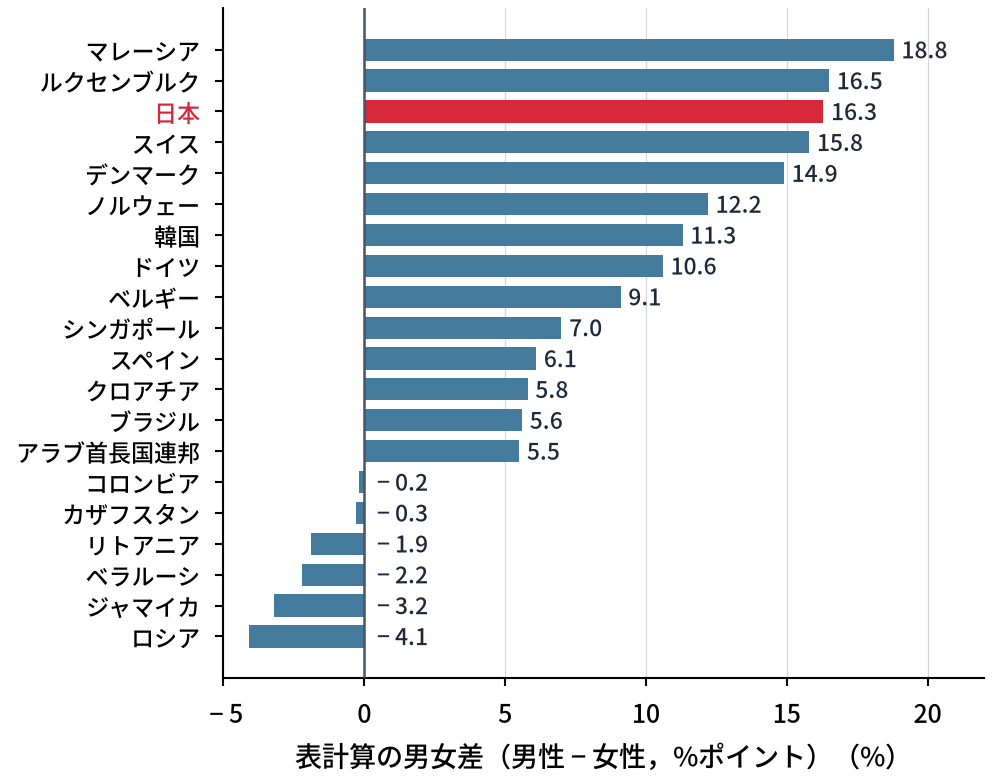
\includegraphics[width=\columnwidth]{chart_unesco_world_ict_skills.png}\caption{表計算の男女差（男性−女性，\%ポイント）の値の比較（上位・下位と日本を抜粋）．赤が日本}\end{figure}
\begin{figure}[t]\centering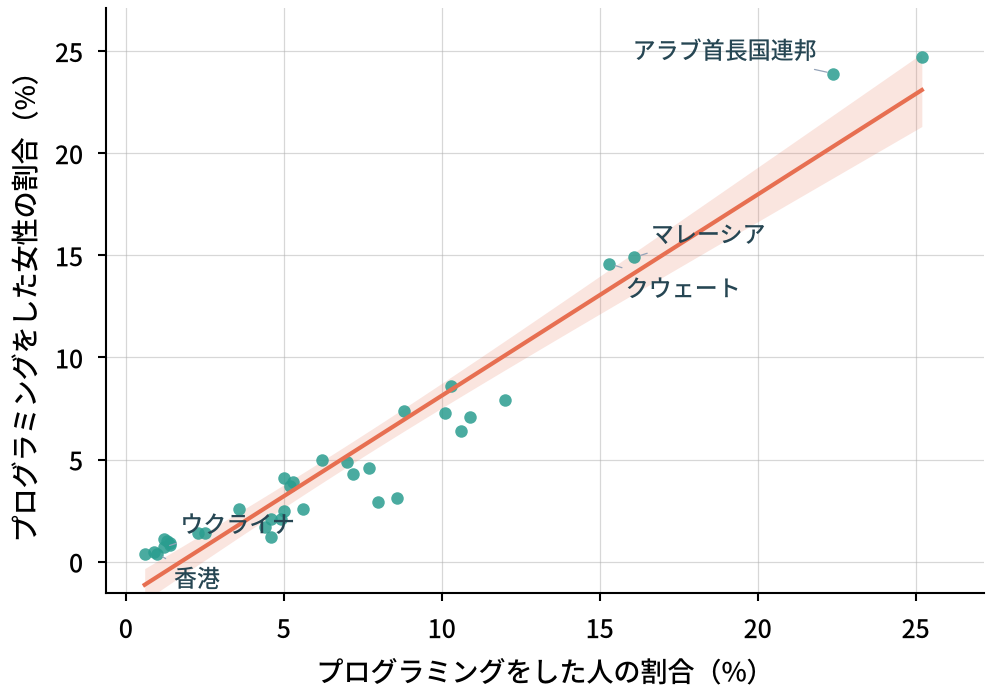
\includegraphics[width=\columnwidth]{chart_secondary_unesco_world_ict_skills.png}\caption{プログラミングをした人の割合とプログラミングをした女性の割合の関連（回帰直線と，その平均の95\%信頼区間の帯，n=36）}\end{figure}
\section{考察}
RQ1では，2つの男女差は国・地域によって大きく異なり，多くの国・地域で男性のほうが高かったが，プレゼン資料作成では女性のほうが高い国・地域も11あり，一方向の現象ではない．日本は両方で男女差が大きい側にあり，プレゼン資料作成では3番目との開きが大きい．ただし日本の女性の割合は表計算で平均を上回っており，男女差の大きさは女性が低いことを意味しない．男性が高いことと合わせて読む必要がある．RQ2では，2つの男女差に正の関連があり，日本やマレーシア，クウェート，小規模な地域を除いても，1か国ずつ除いても残った．対照のプログラミング経験の割合との相関は小さく，表計算の男女差とは\textit{BF}\textsubscript{10}が1/3から3の間でどちらとも言えず，プレゼン資料作成の男女差とは\textit{BF}\textsubscript{10}が1/3未満で関連がないことを支持した．これは国どうしの集計値の関連であり，個々の若者・成人の因果や理由は示さない（生態学的誤謬）．

理由として，デジタル資本（Ragnedda，2018）やデジタルデバイド（van Dijk，2020）をめぐる議論，UNESCO (2023)が問う技術の使われ方，国による情報教育の位置づけの違い（Hubwieser et al.，2015）が考えられる．教える側の知識（Shulman，1986）や，資格が十分でない教員の問題（Ingersoll，1999）が関わる可能性も挙げられる．いずれも仮説にとどまり，本研究のデータでは検証できない．元の統計はITU (2023)が各国の調査から集めたもので，本研究は国・地域ごとの調査の違いを調整していない．

限界は，(1)集計値のみで個人の因果を特定できないこと，(2)元の統計は国によって調査の設計や対象年齢の範囲が異なり，自己申告であること，(3)標本抽出の注意や調査の規模を元データから確かめられないこと，(4)アフリカやオセアニアの国が少なく，男女別の値がない9か国は除かれていること，(5)経済水準や教育条件などの交絡を統制していないこと，(6)2021年の1時点であること，(7)42組の探索で多重比較の影響が残ること，である．教育現場で男女差に取り組む効果は，確かめられていない．
\section*{参考文献}
\begingroup\scriptsize\raggedright\interlinepenalty=10000 
\begin{list}{}{\setlength{\leftmargin}{1.5\zw}\setlength{\itemindent}{-1.5\zw}\setlength{\labelwidth}{0pt}\setlength{\labelsep}{0pt}\setlength{\itemsep}{1pt}\setlength{\parsep}{0pt}\setlength{\topsep}{0pt}\setlength{\listparindent}{0pt}}
\item HUBWIESER, P., GIANNAKOS, M. N., BERGES, M., BRINDA, T., DIETHELM, I., MAGENHEIM, J., PAL, Y., JACKOVA, J. and JASUTE, E. (2015) A global snapshot of computer science education in K-12 schools. Proceedings of the 2015 ITiCSE on Working Group Reports, 65-83.
\item INGERSOLL, R. M. (1999) The problem of underqualified teachers in American secondary schools. Educational Researcher, \textbf{28} (2) ：26-37.
\item ITU (2023) Measuring digital development: Facts and figures 2023. International Telecommunication Union, Geneva.
\item RAGNEDDA, M. (2018) Conceptualizing digital capital. Telematics and Informatics, \textbf{35} (8) ：2366-2375.
\item SHULMAN, L. S. (1986) Those who understand: Knowledge growth in teaching. Educational Researcher, \textbf{15} (2) ：4-14.
\item UNESCO (2023) Global Education Monitoring Report 2023: Technology in Education - A Tool on Whose Terms? UNESCO Publishing, Paris. DOI: 10.54676/aatw1274
\item VAN DIJK, J. (2020) The digital divide. Polity Press, Cambridge.
\item WING, J. M. (2006) Computational thinking. Communications of the ACM, \textbf{49} (3) ：33-35.
\end{list}\endgroup
\section*{Summary}
{\footnotesize\setlength{\parindent}{0pt}Using published 2021 UNESCO Institute for Statistics data, we compared the gender gap (male minus female, percentage points) in spreadsheet and presentation-software use across countries and economies. Among 38 with computable gaps, the spreadsheet gap ranged from −4.1 to 18.8 and the presentation gap from −14.9 to 17.4. Japan ranked 3rd (16.3) and 2nd (15.0), respectively. The two gaps were positively related across 36 countries and economies (r = .75, 95\% CI [0.57, 0.87], BF10 > 1000), and the association remained after excluding Japan and Malaysia (r = .63). These are country-level aggregates and do not imply causation for individuals.\par\smallskip KEYWORDS: UNESCO, ICT Skills, Gender Gap, International Comparison\par}
\medskip\noindent\fbox{\parbox{\dimexpr\columnwidth-2\fboxsep-2\fboxrule}{\footnotesize\gtfamily 【付記：生成AIによる自動執筆に関する開示】\\ 本論文は学生への教育目的で作成している．使用しているデータは公的オープンデータである．統計の算出はPythonで行い，文章は生成AI（Anthropic Claude等）を活用して作成した．記載した統計数値は元データに準拠しているが，教育学的な考察や提言の妥当性は，指導現場の実情に応じて，批判的に吟味してほしい．}}
\end{document}
